\documentclass[
 size=12pt,
 paper=smartboard, %a4paper, smartboard, screen
 mode=present, %present, handout, print
 display=slides, % slidesnotes, notes, slides
 style=tuliplab,  % TULIP Lab style
 pauseslide,
 fleqn,leqno,clock]{powerdot}

\usepackage{amssymb}
\usepackage{amsmath}
\usepackage{rotating}
\usepackage{graphicx}
\usepackage{epstopdf}
\usepackage{boxedminipage}
\usepackage{media9}
\usepackage{rotate}
\usepackage{calc}
\usepackage[absolute]{textpos}
\usepackage{psfrag,overpic}
\usepackage{fouriernc}
\usepackage{pstricks,pst-node,pst-text,pst-3d,pst-grad}
\usepackage{moreverb,epsfig,color,subfigure}
\usepackage{color}
\usepackage{pstricks}
\usepackage{pstricks-add}
\usepackage{pst-text}
\usepackage{pst-node, pst-tree}
\usepackage{booktabs}
\usepackage{etex}
\usepackage{breqn}
\usepackage{multirow}
% \usepackage{pst-rel-points}
\usepackage{listings}
\usepackage{hyperref}
\hypersetup{ % TODO: PDF meta Data
  pdftitle={Presentation Title},
  pdfauthor={Gang Li},
  pdfpagemode={FullScreen},
  pdfborder={0 0 0} 
}


% \usepackage{auto-pst-pdf}
% package to show source code

\definecolor{LightGray}{rgb}{0.9,0.9,0.9}
\newlength{\pixel}\setlength\pixel{0.000714285714\slidewidth}
\setlength{\TPHorizModule}{\slidewidth}
\setlength{\TPVertModule}{\slideheight}
\newcommand\highlight[1]{\fbox{#1}}
\newcommand\icite[1]{{\footnotesize [#1]}}

\newcommand\twotonebox[2]{\fcolorbox{pdcolor2}{pdcolor2}{#1\vphantom{#2}}\fcolorbox{pdcolor2}{white}{#2\vphantom{#1}}}
\newcommand\twotoneboxo[2]{\fcolorbox{pdcolor2}{pdcolor2}{#1}\fcolorbox{pdcolor2}{white}{#2}}
\newcommand\vpspace[1]{\vphantom{\vspace{#1}}}
\newcommand\hpspace[1]{\hphantom{\hspace{#1}}}
\newcommand\COMMENT[1]{}

\newcommand\placepos[3]{\hbox to\z@{\kern#1
        \raisebox{-#2}[\z@][\z@]{#3}\hss}\ignorespaces}


%%%%%%%%%%%%%%%%%%%%%%%%%%%%%%%%%%%%%%%%%%%%%%%%%%%%%%%%%%%%%%%%%%%%%%%%%%
%%% title
%%% TODO: Customize to your Own Title, Name, Address
%%%
\title{FLIP(01) Mid-term Presentation}
\author{Rongxin Xu\\
Hunan University
% \href{mailto:gangli@acm.org}{gangli@acm.org}
% \and % more authors
}
\date{19 January 2019}



% Customize the setting of slides
\pdsetup{
% TODO: Customize the left footer, and right footer
rf={\copyright \emph{FLIP(01)}},
cf={FLIP(01) Presentation },
}


% Starts the document
\begin{document}

\maketitle

%%==========================================================================================
%%
\begin{slide}[toc=,bm=]{Outline}
  \tableofcontents[content=sections]
\end{slide}
%%
%%==========================================================================================

\section{Introduction}

\begin{slide}{Problem Description}
  \begin{itemize}
    \item
		The ubiquitousness of smartphones enables 
		people to announce an emergency they’re 
		observing in real-time. 
          \begin{itemize}
            \item
				Predict whether a real disaster has occurred 
				based on keywords, location, and Twitter text.
          \end{itemize}
  \end{itemize}
\end{slide}

\section{Data Description}
%
\begin{slide}{Attribute Information}
  \begin{itemize}
    \item<1->
          Attributes Information
    \item[1.]
          There are 3 data sets.
    \begin{description}
    	\item[train.csv] the training set.
    	\item[test.csv] the test set.
    	\item[sample\_submission.csv] a sample submission file in the correct format.
    \end{description}
    \item[2.]
          There are 3 data sets with a total of 5 attributes.
\end{itemize}
\begin{table}[htbp]
	\centering
	\caption{Attribute Information}
	\begin{tabular}{llllll}
	\hline
	% after \\: \hline or \cline{col1-col2} \cline{col3-col4} ...
	Attributes & Information                                                                            \\
	\hline
	id   & a unique identifier for each tweet                                                               \\
	text    & the text of the tweet                                                                         \\
	location     & the location the tweet was sent from (may be blank)                                      \\
	keyword     & a particular keyword from the tweet (may be blank)                                        \\
	target    &  in train.csv only, this denotes whether a tweet is about a real disaster (1) or not (0)    \\                                               \\
	\hline
	%\bottomrule
\end{tabular}
\end{table}
\end{slide}


\section{Exploratory Data Analysis}

\begin{slide}{Scatter plot of keywords}
  \begin{figure}[htbp]
    \centering
      \includegraphics[width=.7\linewidth,height=.5\linewidth]{Figures/scatter_keywords.eps}
    \caption{Scatter plot of keywords}
  \end{figure}
\end{slide}

\begin{slide}{Scatter plot of location}
  \begin{figure}[htbp]
	\centering
	\includegraphics[width=.7\linewidth,height=.5\linewidth]{Figures/scatter_location.eps}
	\caption{Scatter plot of location}
  \end{figure}
\end{slide}


\begin{slide}{Missing Values}
  \begin{figure}
    \centering
    % Requires \usepackage{graphicx}
    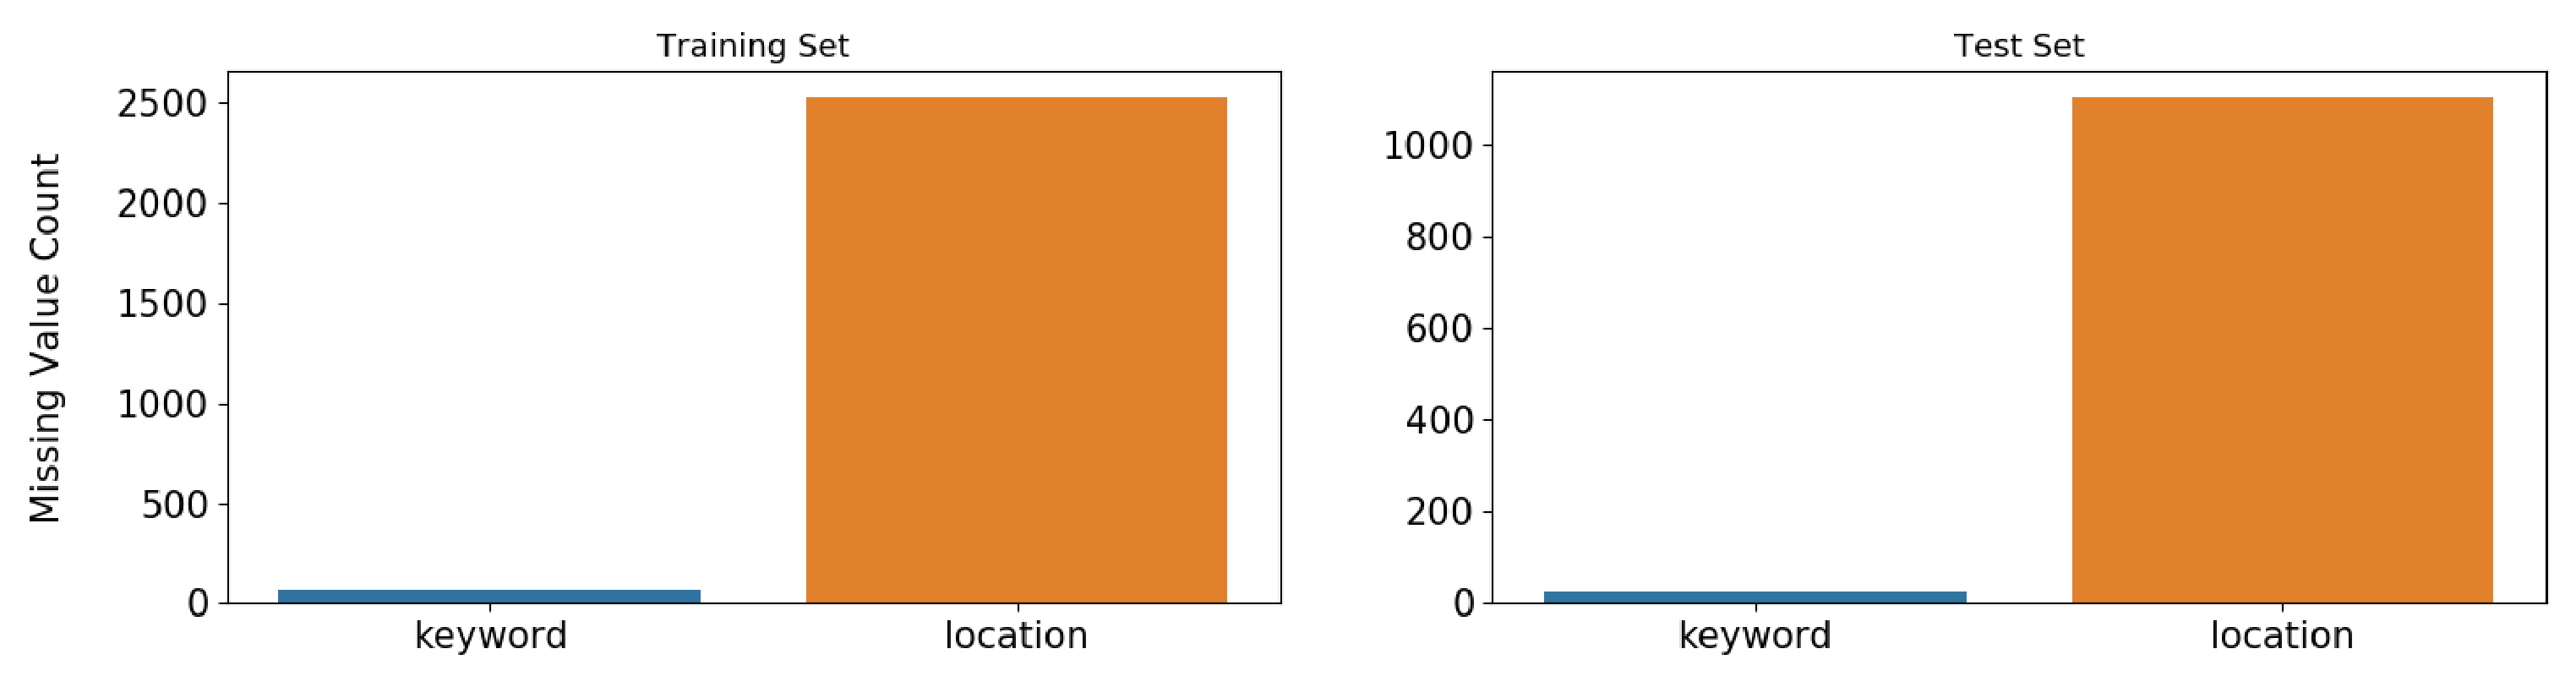
\includegraphics[width=.9\linewidth,height=.3\linewidth]{Figures/hits.eps}
    \caption{Missing Values of location and keywords}
  \end{figure}
\end{slide}

\begin{slide}{Summary}
  \begin{itemize}
	\item<1->
	Both training and test set have same ratio of missing values in keyword and location.
	\item[1.]
	0.8\% of keyword is missing in both training and test set.
	\item[2.]
	33\% of location is missing in both training and test set.
	~\\
	~\\
	\item<1->
	From Data description and above analysis we can conclude :
	\item[1.]
	Locations are not automatically generated, they are user inputs and that's why data is not clean and there are too many incoorect and missing values.We can skip the 'location' column from our feature list.
	\item[2.]
	We can consider the 'keyword' column as a feature because there are a lot of unique keywords and missing values are very insignificant (< 1 percentage).
\end{itemize}
\end{slide}

\section{Data Preprocessing}
\begin{slide}{Basic NLP Techniques}
	Create a Corpus from 'Text' coloumn, Corpus is a simplified version of our text data that contain clean data. To create Corpus should have to perform the following actions
	\begin{description}
	\item[Remove unwanted words] Removal of unwanted words such as special characters and numbers to get only pure text.
	\item[Transform words to lowercase] Transform words to lowercase because upper and lower case have diffirent ASCII codes.
	\item[Remove stopwords] Stop words are usually the most common words in a language and they will be irrelevant in determining the nature.
	\item[Stemming words] Stemming is the process of reducing words to their word stem, base or root form.
	\end{description}
\end{slide}

\section{Modeling and Model Evaluation}
\begin{slide}{Evaluation}
	Use F1 score.
  \begin{itemize}
    \item
          F1 is calculated as follows: \\[10 pt]
		$F _ { 1 } = 2 * \frac { \text { precision } * \text { recall } } { \text { precision } + \text {recall} }$
\\[10 pt]
    \item
		where: \\[10 pt]
		$\begin{aligned} \text {precision} & = \frac { T P } { T P + F P } \\ \text {recall} & = \frac { T P } { T P + F N } \end{aligned}$
  \end{itemize}
\end{slide}

\begin{slide}{Modeling}
	Since this NLP problem is also a binary classification problem, we might as well try some traditional classification models, such as:
		\begin{description}
	\item[Gaussian Naive Bayes]
	\item[Gradient Boosting]
	\item[K - Nearest Neighbor]
	\item[Decision Tree]
	\item[Logistic Regression]
	\item[XGBOOST]
	\item[Voting Classifier]
\end{description}
\end{slide}

\begin{slide}{Model Evaluation}
	Use F1 score and accuracy to evaluate model performance.
% Table generated by Excel2LaTeX from sheet 'Sheet1'
\begin{table}[htbp]
	\centering
	\caption{Model Evaluation}
	\begin{tabular}{llll}
		\toprule
		\multicolumn{1}{c}{model} & \multicolumn{2}{c}{Accuracy Score} & \multicolumn{1}{c}{F1 Score} \\
		& \multicolumn{1}{c}{Train Data Set} & \multicolumn{1}{c}{Test Data Set} &  \\
		\midrule
		\textbf{Gaussian Naive Bayes} & 0.783314021 & 0.75843812 & 0.653371 \\
		\textbf{Gradient Boosting} & 0.853666611 & 0.75446724 & 0.647673 \\
		\textbf{K - Nearest Neighbors} & 0.975004138 & 0.726009265 & 0.56051 \\
		\textbf{Decision Tree} & 0.975004138 & 0.729318332 & 0.663374 \\
		\textbf{Logistic Regression} & 0.840258235 & 0.80344143 & 0.752706 \\
		\textbf{XGBOOST} & 0.840258235 & 0.80344143 & 0.752706 \\
		\textbf{Voting Classifier} & 0.898857805 & 0.782925215 & 0.752706 \\
	\end{tabular}%
\end{table}%
\end{slide}


\section{Conclusion and Future research}
\begin{slide}{Conclusion}
  \begin{itemize}
    \item 	Locations are not automatically generated, they are user inputs and that's why data is not clean and there are too many incoorect and missing values.We can skip the 'location' column from our feature list.
          \bigskip
    \item In traditional classification models, the logistic regression model, XGBOOST, and Voting Classifier have higher F1 scores, which means that the performance is better than other models.
  \end{itemize}
\end{slide}

\begin{slide}{Future research}
  \begin{itemize}
    \item Embeddings \& Text Cleaning.
    \item Design meta features and extract features using N-gram.
    \item Use word2vec, glove, BERT, etc. to construct word vectors and compare their performance.
  \end{itemize}
\end{slide}

\begin{wideslide}[toc=,bm=]{}
  \centering
  \vspace{\stretch{1}}
  \twocolumn[
    lcolwidth=0.35\linewidth,
    rcolwidth=0.65\linewidth
  ]
  {
    % \centerline{\includegraphics[scale=.2]{tulip-logo.eps}}
  }
  {
    \vspace{\stretch{1}}


    \textcolor{black}{\scalebox{2.0}{Thank you \& Question}}


  }
  \vspace{\stretch{1}}
\end{wideslide}

\end{document}
\endinput
